\chapter{Introduction}
\label{chap:intro}

%%%%%%%%%%%%%%%%%%%%%%%%%%%%%%%%%%%%%%%%%%%%%%%%%%%%%%%%%%%%%%%%%%%%%%%%%%%%%%%
\section{Background}
\label{sec:chap1-background}


\begin{figure}
\begin{subfigure}{.5\textwidth}
  \centering
  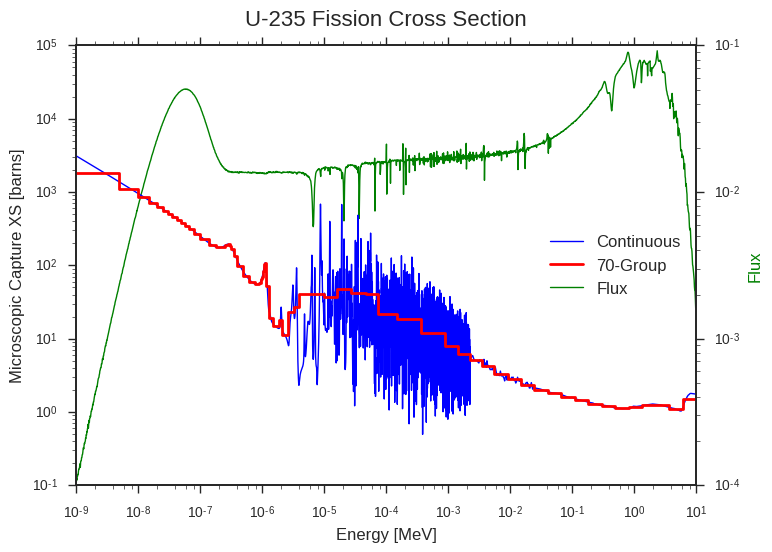
\includegraphics[width=\linewidth]{figures/intro/u235-fission-70}
  \caption{}
  \label{fig:assm-cells}
\end{subfigure}%
\begin{subfigure}{.5\textwidth}
  \centering
  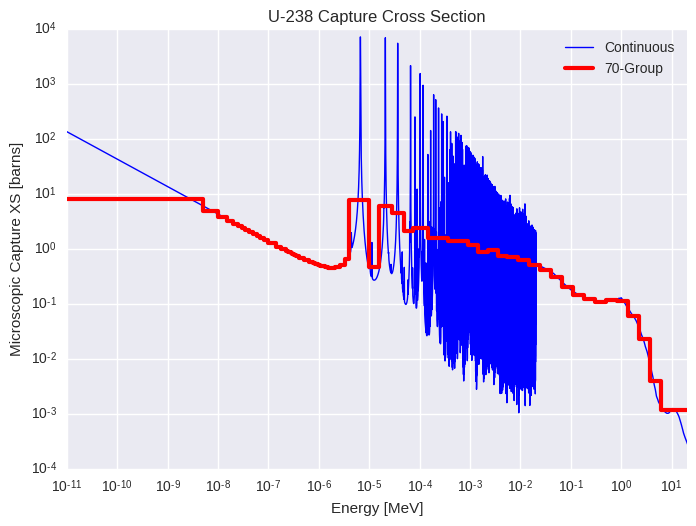
\includegraphics[width=\linewidth]{figures/intro/u238-capture-70}
  \caption{}
  \label{fig:colorset-cells}
\end{subfigure}
\begin{subfigure}{.5\textwidth}
  \centering
  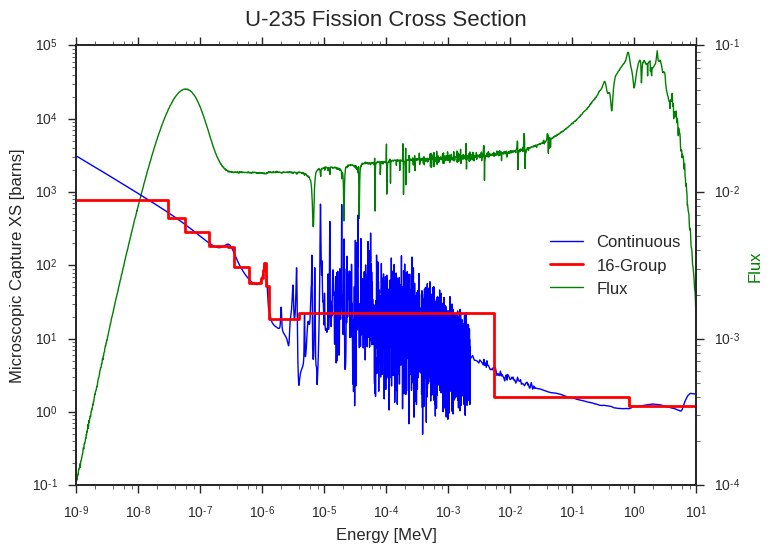
\includegraphics[width=\linewidth]{figures/intro/u235-fission-16}
  \caption{}
  \label{fig:assm-unique-neighbors}
\end{subfigure}
\begin{subfigure}{.5\textwidth}
  \centering
  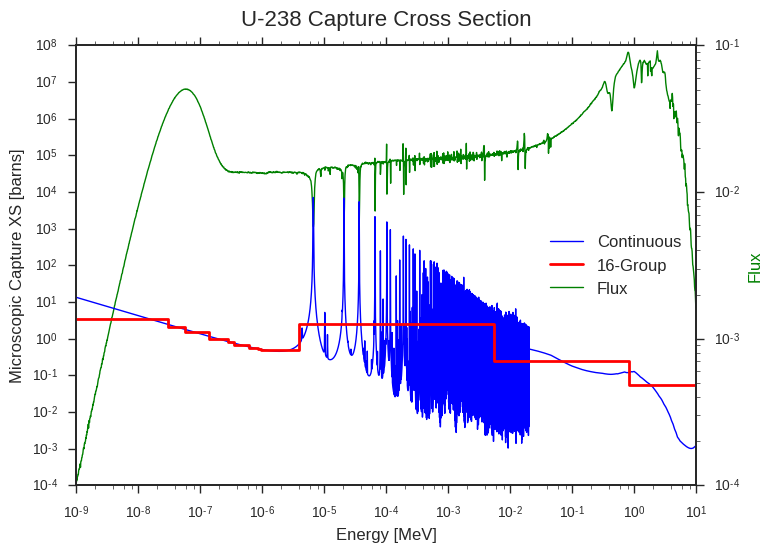
\includegraphics[width=\linewidth]{figures/intro/u238-capture-16}
  \caption{}
  \label{fig:colorset-unique-neighbors}
\end{subfigure}
\begin{subfigure}{.5\textwidth}
  \centering
  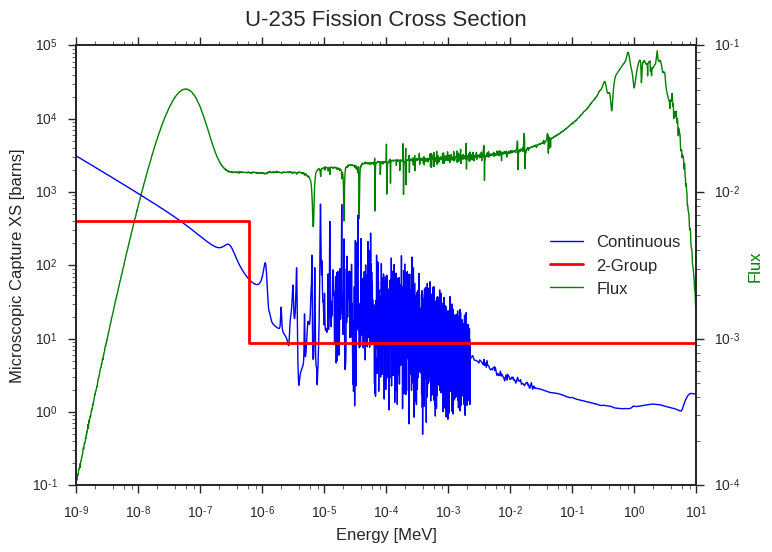
\includegraphics[width=\linewidth]{figures/intro/u235-fission-2}
  \caption{}
  \label{fig:assm-neighbors}
\end{subfigure}
\begin{subfigure}{.5\textwidth}
  \centering
  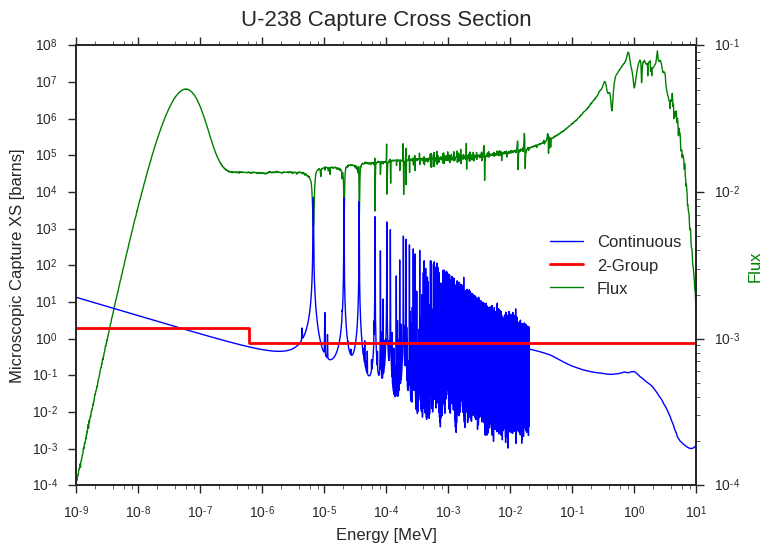
\includegraphics[width=\linewidth]{figures/intro/u238-capture-2}
  \caption{}
  \label{fig:colorset-neighbors}
\end{subfigure}
\caption{Continuous energy and multi-group cross sections for U-235 fission (left) and U-238 capture (right) reactions in a PWR spectrum for 70-, 16- and 2-groups.}
\label{fig:pwr-ce-mg-xs}
\end{figure}


%%%%%%%%%%%%%%%%%%%%%%%%%%%%%%%%%%%%%%%%%%%%%%%%%%%%%%%%%%%%%%%%%%%%%%%%%%%%%%%
\section{High-Performance Computing Trends}
\label{sec:chap1-hpc-trends}


%%%%%%%%%%%%%%%%%%%%%%%%%%%%%%%%%%%%%%%%%%%%%%%%%%%%%%%%%%%%%%%%%%%%%%%%%%%%%%%
\section{Whole-Core Neutron Transport Simulations}
\label{sec:chap1-whole-core-transport}


%%%%%%%%%%%%%%%%%%%%%%%%%%%%%%%%
\subsection{Monte Carlo Methods}
\label{subsec:chap1-monte-carlo}


%%%%%%%%%%%%%%%%%%%%%%%%%%%%%%%%%%
\subsection{Deterministic Methods}
\label{subsec:chap1-deterministic}

\begin{itemize}
  \item 2D/1D methods in MPACT, nTracer
  \item Denovo, PDT, 3D OpenMOC, etc.
\end{itemize}


%%%%%%%%%%%%%%%%%%%%%%%%%%%%%%%%%%%%%%%%%%%%%%%%%%%%%%%%%%%%%%%%%%%%%%%%%%%%%%%
\section{Multi-Group Cross Sections}
\label{sec:chap1-mgxs}

\begin{itemize}[noitemsep]
  \item black magic ``crux'' of deterministic methods
  \item need accurate \ac{MGXS} for whole core transport methods
  \item motivate \ac{MC} for \ac{MGXS}
\end{itemize}